%%%%%%%%%%%%%%%%%%%%%%%%%%%%%%%%%%%%%%%%%%%%%%%%%%%%%%%%%%%%%%%%%%%%%%%%%%%%%%%%
% experiment.tex: Chapter describing the experiment
%%%%%%%%%%%%%%%%%%%%%%%%%%%%%%%%%%%%%%%%%%%%%%%%%%%%%%%%%%%%%%%%%%%%%%%%%%%%%%%%
\chapter{The NOvA Experiment}
\label{experiment_chapter}
%%%%%%%%%%%%%%%%%%%%%%%%%%%%%%%%%%%%%%%%%%%%%%%%%%%%%%%%%%%%%%%%%%%%%%%%%%%%%%%%

The neutrinos studied by NOvA begin at Fermi National Accelerator Laboratory (Fermilab) 
in Illinois.  An intense muon (anti-)neutrino beam is created at Fermilab by the Neutrino 
at the Main Injector (NuMI) source. NOvA, which stands for NuMI Off-Axis $\nu_e$ Appearance, 
is a long baseline experiment which is designed to determine the neutrino mass hierarchy, 
the octant of $\theta_{23}$, and to measure the CP violating phase $\delta_{CP}$ by measuring 
electron (anti-)neutrino appearance probability and muon (anti-)neutrino disappearance. It 
consists of the Near Detector (ND), which is located at Fermilab and measures total flux of 
neutrino, and the Far Detector (FD), which is located near Ash River, Minnesota and measures 
flux of muon and electron neutrinos. The structures of the NuMI source and the Near and 
Far Detectors, and the detector positions relative to the beam axis will be explained in 
the following sections.

\section{NuMI and Off-Axis Detectors Position}
\begin{figure}
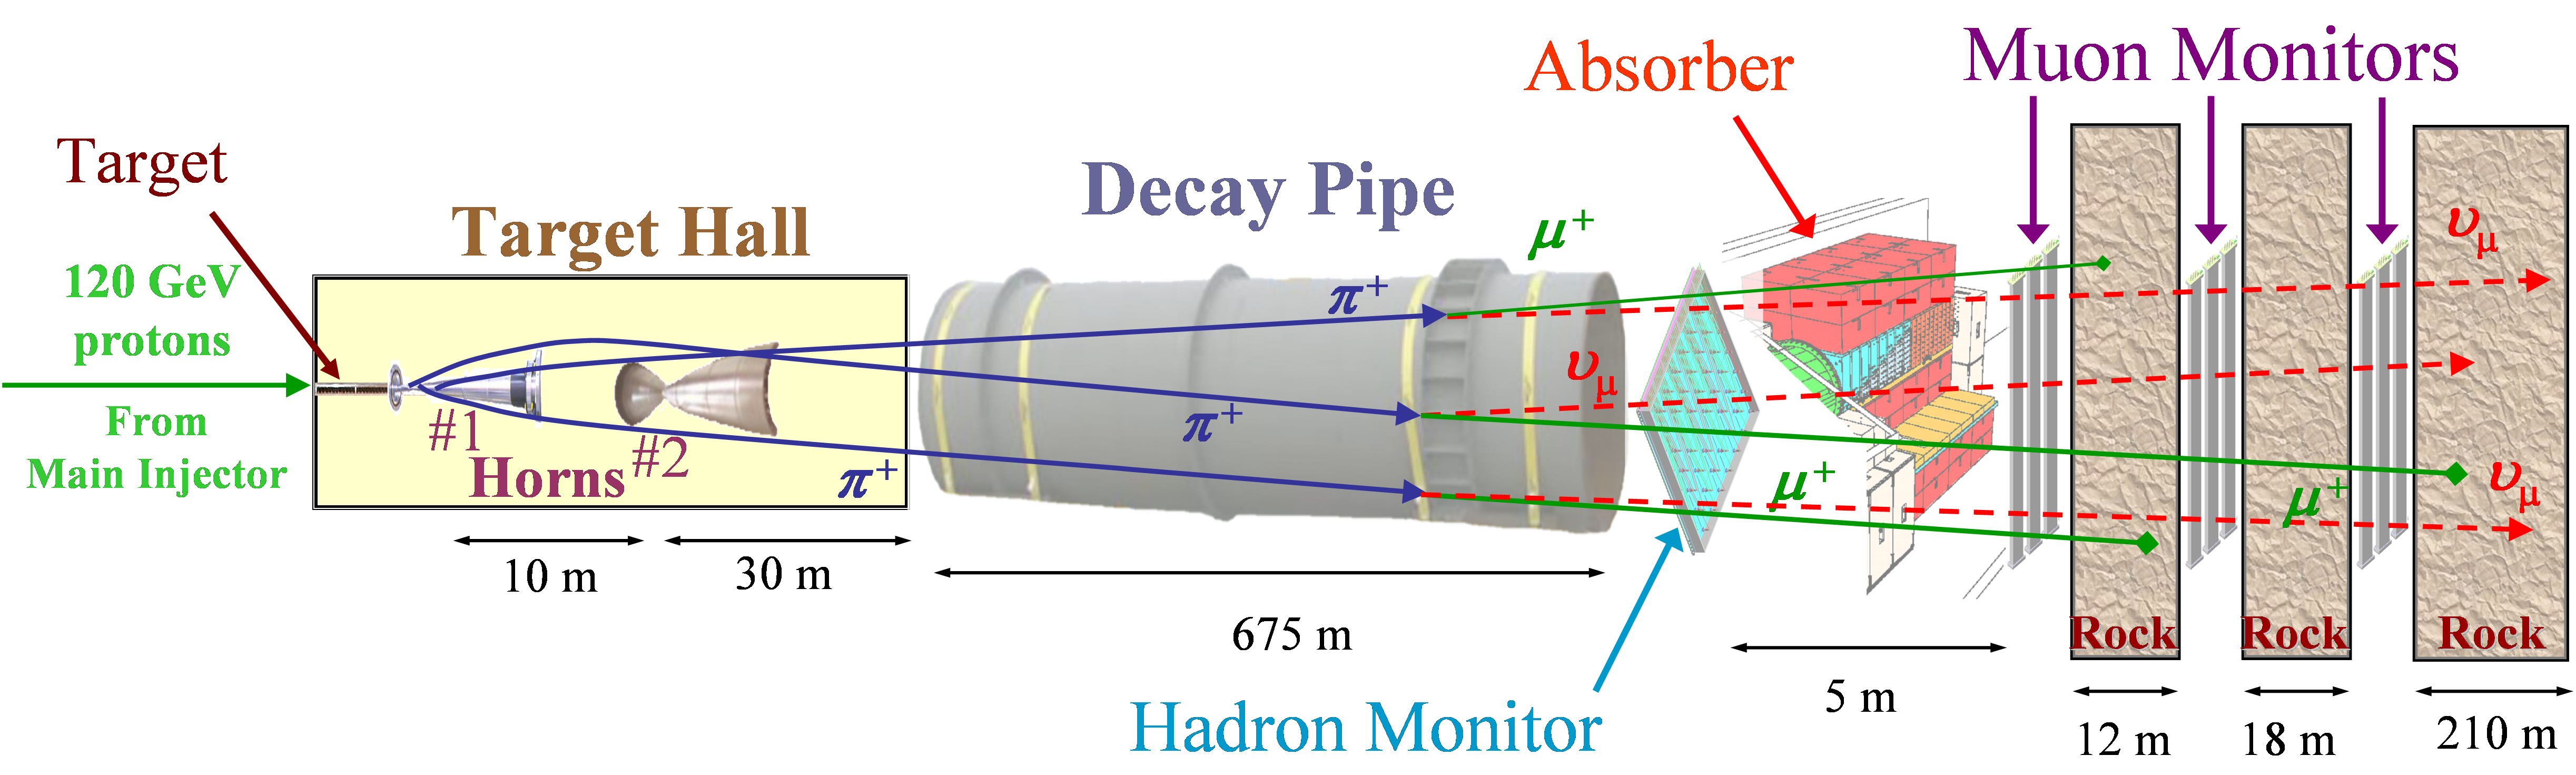
\includegraphics[width=1.0\textwidth]{figures/Beamline.png}
\centering
\caption{Schematics of neutrino production\cite{numi}.} \label{NuMI}
\end{figure}
Neutrinos for the NOvA experiments comes from decay of pions and kaons. To get a beam of 
the mesons Main Injector at Fermilab is used, which provides an intense beam of proton with 
energy 120 GeV. The structure of NuMI is illustrated on figure \p{NuMI}. It is designed to 
deliver $4.9 \times 10^{13}$ proton on target (POT) with the repetition rate of 1.3s, which 
corresponds to 700 kW of beam power. The proton beam is directed into a graphite target.  
Collisions between the proton beam and graphite target produces many types of hadrons and 
mesons, with pions and kaons among them. Magnetic focusing horns, which are supplied with 
current of 200kA, are used to focus and direct 
charged pions and kaons into a decay pipe. The decay pipe is long enough such that nearly all 
of the incoming pions and kaons decay before the end of the pipe. More than 99\% of all pions 
and 63\% of kaons decay into anti-muon/muon and muon/anti-muon neutrino, so the flux of 
particles at the end of the decay pipe consists of mostly muons and muon anti-neutrinos, or 
their antiparticles. By changing the electric current direction in the focusing horns one can 
switch between positively and negatively charged pions and kaons which enter the decay pipe. 
This gives an opportunity to make two types of neutrino beams - $\nu_\mu$'s and $\bar{\nu}_\mu$'s. 
Unfortunately, 5\% of charged kaons have electron neutrinos among their byproducts, and this 
is an irreducible background for an electron neutrino analysis. All the realitively long lived
charged particles such as muons and electrons do not reach Near Detector as they get absorbed 
in rock. A hadron monitor, absorber and muon monitor are placed at the end of decay pipe 
to better understand beam properties, but they do not play any role in the NOvA experiment.

\begin{wrapfigure}{r}{0.5\textwidth}
\vspace{-20pt}
  \begin{center}
    \includegraphics[width=0.48\textwidth]{figures/Neutrino_osc.png}
  \end{center}
\vspace{-30pt}
\end{wrapfigure}

After the neutrinos leave the decay pipe they begin their journey to the near and far detectors. 
There are a few reasons why the NO$\nu$A detectors are placed 14.6 mrad off-axis of the NuMI beam. 
As can be seen on the picture on the right, the first minimum of muon neutrino survival 
probability and first maximum of electron neutrino appearance probability are around 400 km/GeV 
but on-axis neutrino spectrum (black line on left picture \p{Spec}) does not allow to observe 
first maximum of $P(\nu_\mu \rightarrow \nu_e)$ for a baseline $~1000$ km. The solution is 
simple: pions and kaons decay isotropically in their rest frame but after Lorentz boost to 
laboratory frame flux and neutrino energy at the far detector (for small off-axis angles $\theta$) 
can be expressed in the following form
\be
F = \Big(\frac{2\gamma}{1+\gamma^2\theta^2}\Big)^2\frac{A}{4\pi d}
\ee
\be
E_\nu = \frac{0.43E_\pi}{1+\gamma^2\theta^2},
\ee
where $\gamma = \frac{E_\pi}{m_\pi}$, $A$ is the size of the detector front area and $d$ is 
the distance to the detector. For kaons numerical factor $0.43$ should be changed to $0.96$. 
Knowing the pion and kaon energy spectrum at the NuMI source, one can predict the neutrino energy 
spectrum at the far detector for different off-axis angles $\theta$. As shown on left side of 
\autoref{Spec}, the neutrino energy distribution gets narrower and shifts toward smaller energies. 
At 14.6 mrad the neutrino flux is still moderate and peaked near 2 GeV, which allows NOvA 
to study the region of maximal $P(\nu_\mu \rightarrow \nu_e)$ at 810 km. Moreover, the narrow 
peak decreases the chance that NC events from more energetic neutrinos could be misidentified 
as CC events in the energy region of interest. In general, the off-axis detector placement 
significantly improves the sensitivity of the probability measurement.
\begin{figure}
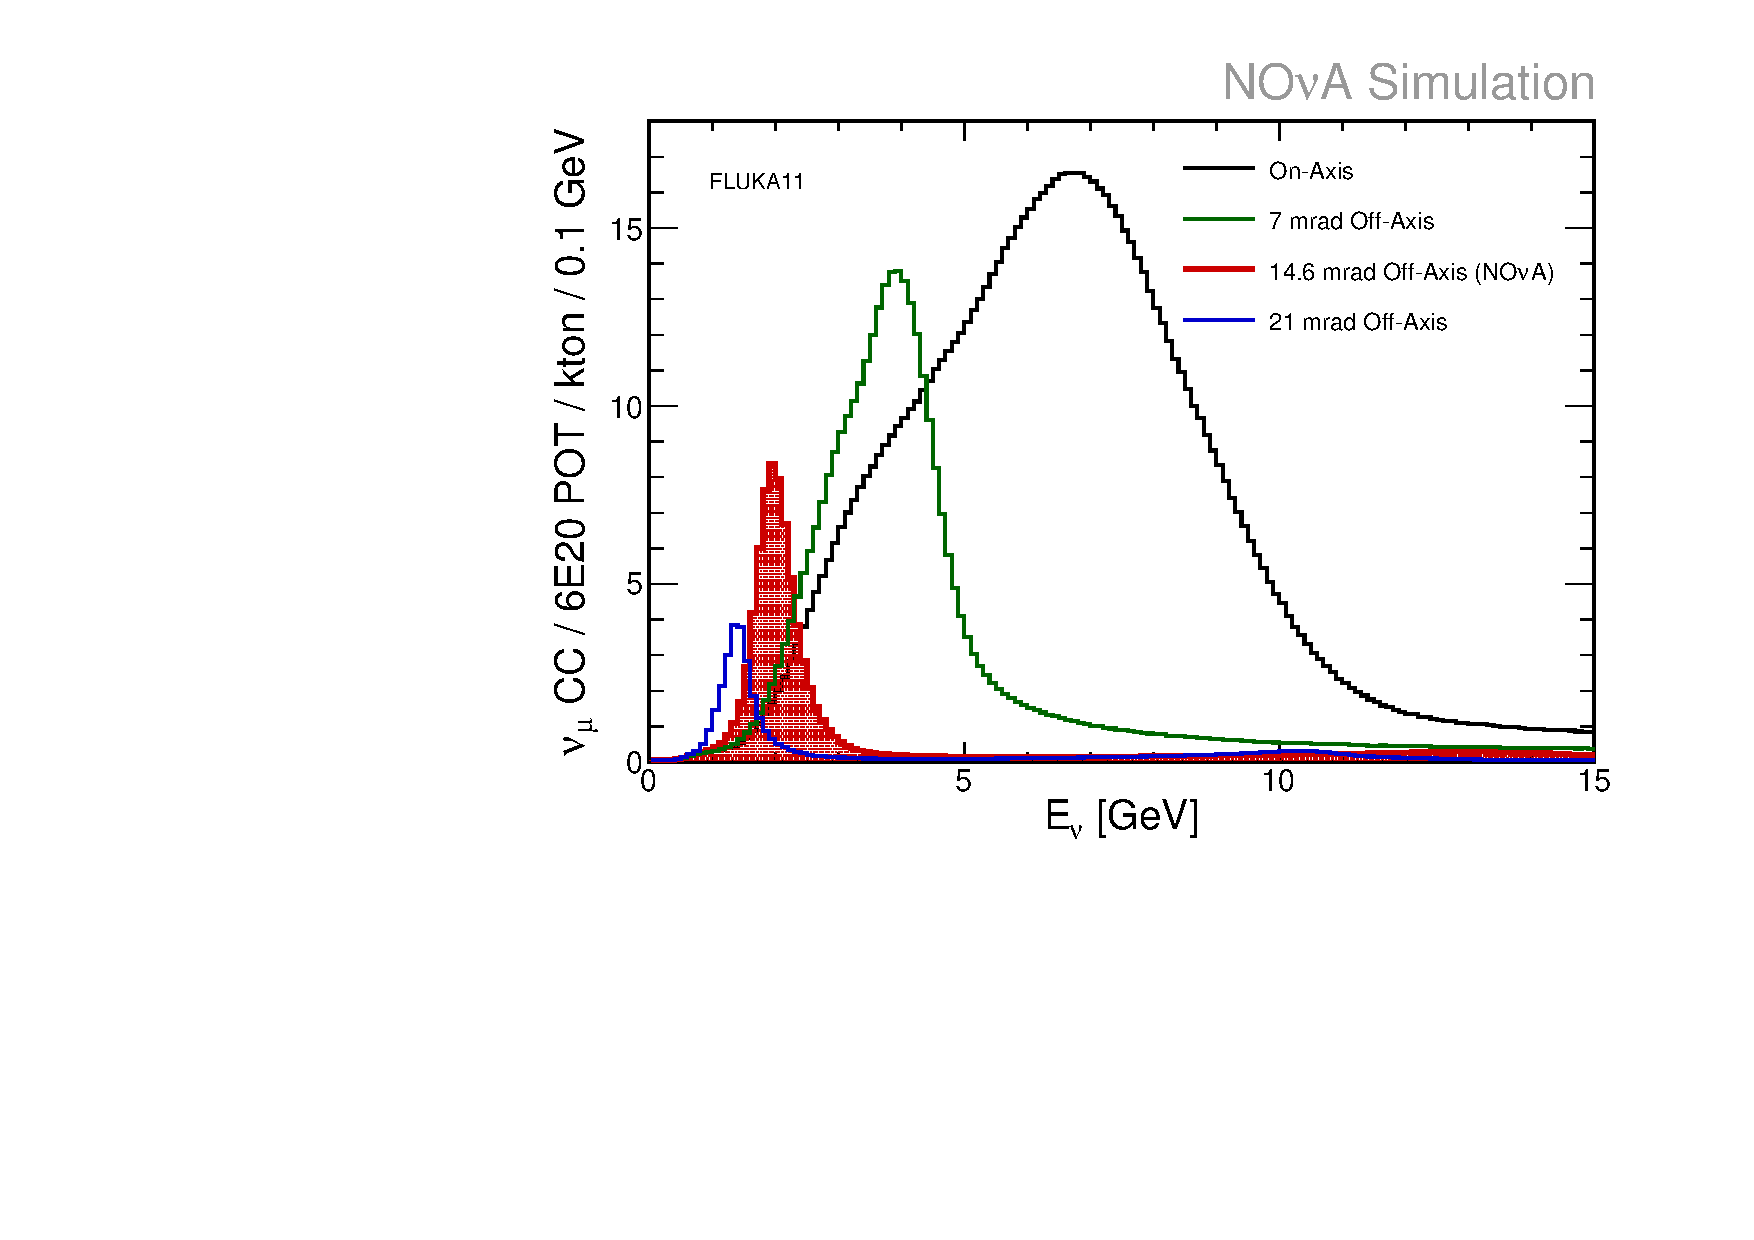
\includegraphics[width=0.9\textwidth]{figures/FD_NOvA_OffAxis_Spectra.pdf}\\%
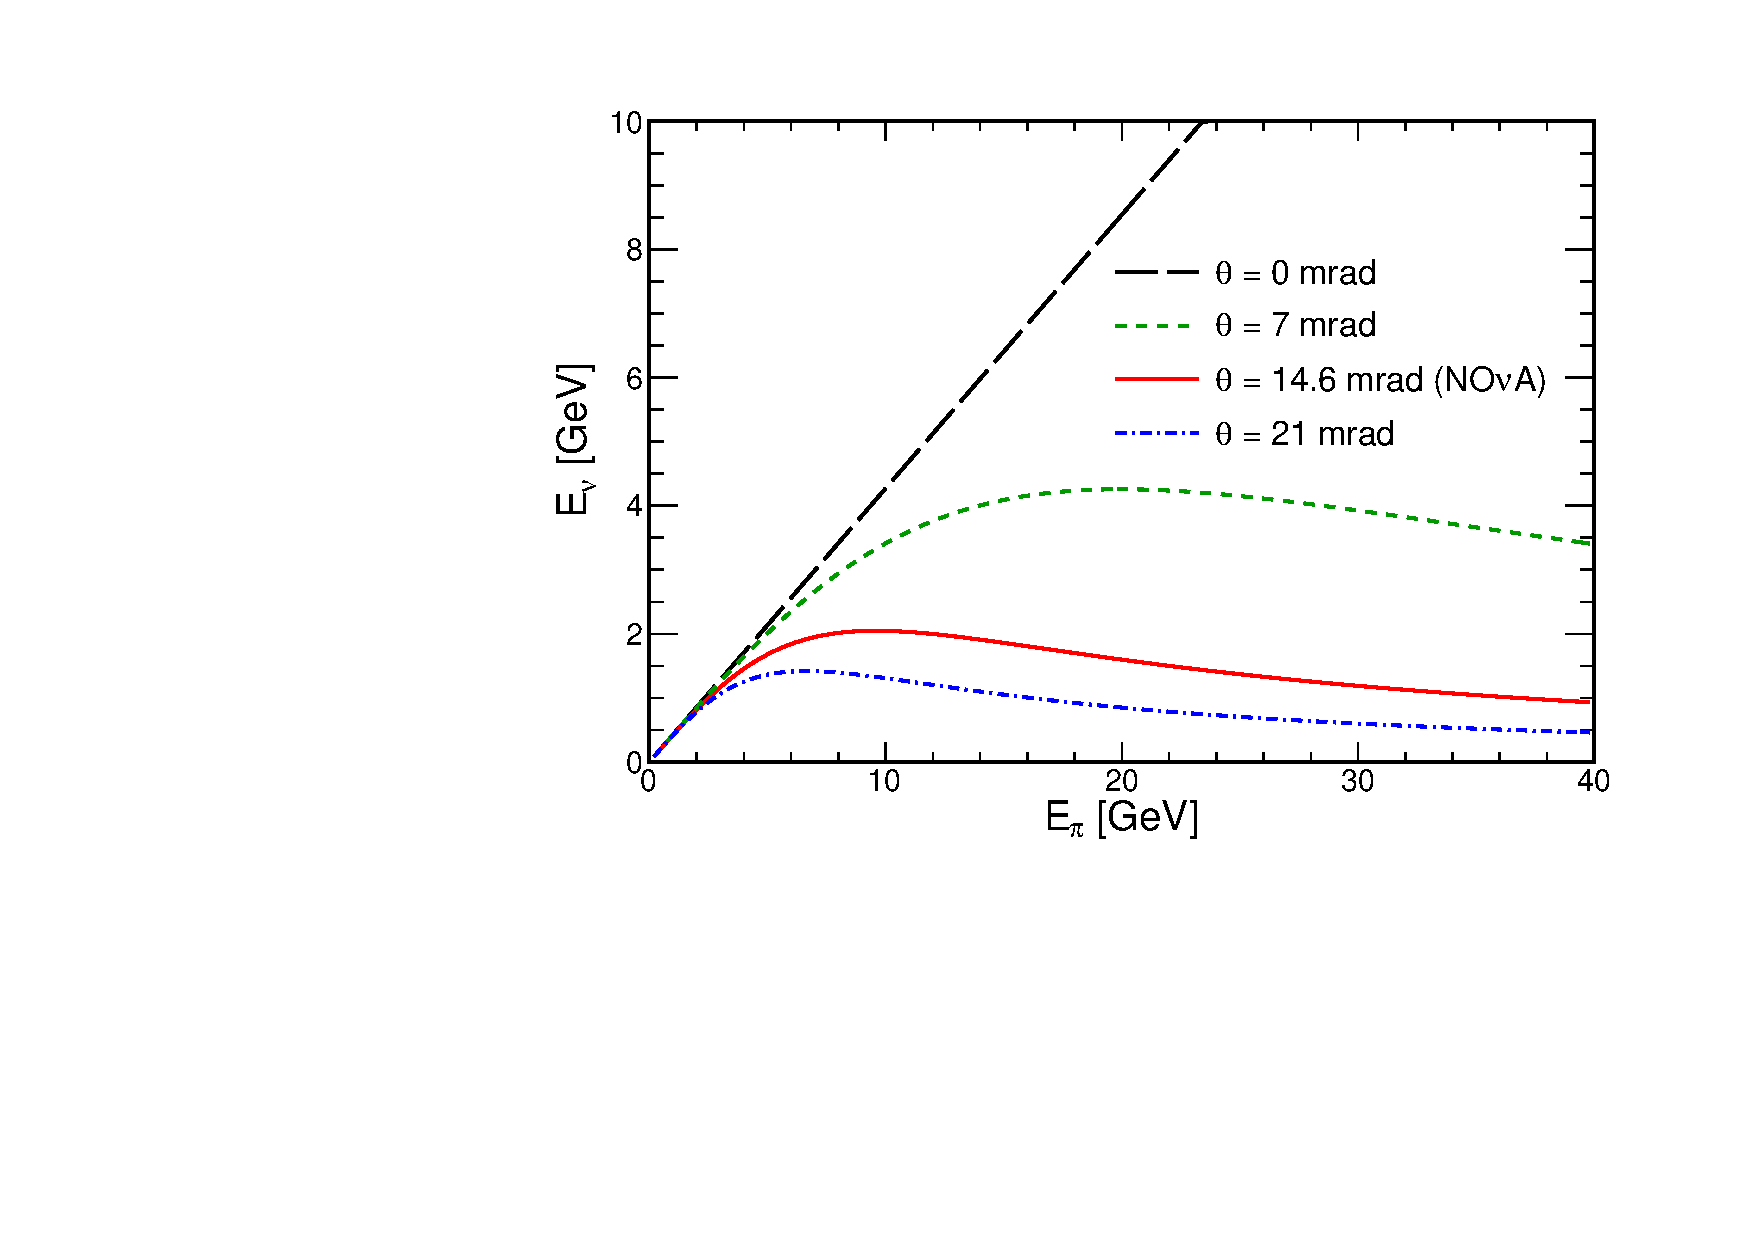
\includegraphics[width=0.9\textwidth]{figures/EnuVSEpi_NOvA.pdf}
\centering
\caption{(Left) Expected unoscillated neutrino spectrum at the Far Detector as a function of 
angle relative to NuMI beam. (Right)~Neutrino oscillation probabilities as a function of $\frac{L}{E}$, $
P(\nu_\mu \rightarrow \nu_\mu)$ - blue line, $P(\nu_\mu \rightarrow \nu_e)$ - black line and 
$P(\nu_\mu \rightarrow \nu_\tau)$ - red line.} \label{Spec}
\end{figure}

\section{NOvA Near and Far Detectors}
The NOvA experiment utilizes two detectors for measuring muon neutrino disappearance probability 
$P(\nu_\mu \rightarrow \nu_\mu)$ and electron neutrino appearance probability $P(\nu_\mu \rightarrow \nu_e)$. 
In order to decrease systematic uncertainties, such as beam uncertainty and uncertainties due to variation
in detector efficiency, two detectors are build with exactly the same material and 
similar geometry. The Near Detector is placed 1 km from the NuMI source at Fermilab, while the 
Far Detector sits 810~km away on the surface and 14.6 mrad off beam axis in Ash River, Minnesota. 
The Near Detector weighs 330 metric ton and is 105 m underground, while the Far Detector mass is 
14,000 ton and has shielding equivalent to 3 m of rock which reduces cosmic ray background.
\begin{figure}
\begin{subfigure}{.2\textwidth}
  \centering
  \includegraphics[width=0.79\linewidth]{figures/PVC_cell_original.jpg}
  \caption{A NOvA cell}
  \label{cell}
\end{subfigure}%
\begin{subfigure}{.8\textwidth}
  \centering
  \includegraphics[width=\linewidth]{figures/2detectors.pdf}
  \caption{Scale and structureof the NOvA detectors}
  \label{2detectors}
\end{subfigure}
\caption{Structure of cell and the NOvA detectors}
\label{cell_detectors}
\end{figure}

\subsection{From cells to planes and blocks}
Each detector is made of cells which are made from polyvinyl chloride (PVC) doped with titanium 
dioxide to increase light reflectivity. The cross section of cells has rectangular shape with sizes
approximately equal to 4 cm and 6 cm. The length of the cells is varies between the detectors and 
equals to 4 m for the Near Detector and 15 m for the Far Detector. 32 cells are bound together along
6 cm side to make a module and the set of modules produces plane. The number of modules in a plane
depends on a detector - 3 and 12 modules per plane for the Near and Far Detector respectively. Planes
are glued together in a such way that adjacent planes alternating between horizontal and vertical
allignment. The scetch of the detectors structure can be seen in \p{2detectors}. Furthemore, 32 planes 
make up a block and 28 blocks complete the full Far Detector while for the Near Detector block consists
of 24 planes and 3 blocks make the active part of the detector. In addition, so called muon catcher
block goes upstream and serves for stopping muons which are produced in $\nu_\mu$ CC interactions. 
Muon catcher, which helps to contain more muons as the relative size of the Near Detector is not big, 
consists of 22 active planes together with 10 steel 10 cm thick planes between every 2 active ones. The size
of the muon catcher in XY plane is smaller the the active part of the Near Detector since horizontal
planes have only 2 modules while vertical planes have 3 modules. The presents of the steel leads to
extra muon energy absorbtion which makes muon tracks shorter.

Planes configuration allows to reconstruct three-dimensional tracks of the particles; vertical cells 
provide X measurements, horizontal cells give Y measurements, and planes positions provides Z measurements. 
Z-axis is directed along the beam, X-axis points to the west and Y-axis points upward. This choice of
axes gives NOvA detectors a Cartesian right handed coordinate system. 

\subsection{Signal path part I: ligth production and digitization}
In order to detect particles resulted in neutrino interactions in the detectors these particles 
should leave footprints. In NOvA experiment cells are filled with a liquid scintillator composed 
of mineral oil doped with pseudocumene~\footnote{1,2,3-Trimethylbenzene}. In every cell, one wavelength 
shifting fiber runs from one end of the cell to the opposite end, then back to the other end where 
it connects to an avalanche photodiode (APD) as can be seen in \p{cell}. Photons are created by charged 
particle moving through the scintillator. These reflected by the cell walls and have a high chance 
to be captured by the wavelength shifting fiber. Inside the fiber photons after absorbtion and
reemission increse its wavelength resulting in propogation without escaping due to total inner
reflection. 

Photons which reach APD get converted into photoelectrons through the process called avalanche 
breakdown, and produces currents which are detectable by commercial electronics. All 32 fiber from
the module are connected to one APD. And the last step before signals might be processed with the 
help of conventional computers is to digitize the APD output signal. The digitization happens in
front end board (FEB). Short APD signals are stretched in time in the Application Specific 
Integrated Circuit (ASIC) with the help of CR-RC circuit. After, the signal is passed to ADC - 
analog to digital converter - where continuous signal is translated to discrete one with 4096 
distinct values. Every channel is read out every 500 ns and 125 ns for the Far and Near Detector 
respectively. Only the 4 last ADCs - value of the digitization sample - are stored as a hit and 
the hit is written when the difference
\be
ADC_i - ADC_{i-3}
\ee
is greater than a threshold. These 4 values are then passed to the Data Concentration Module (DCM). 
Later, those 4 values are used to fit the signal shape and to determine signal amplitude, which 
is proportional to amount of energy charged particle deposited in a particular cell.

\subsection{Signal path part II: data acquisition}
Every DCM is a custom built computer and collecting data from 64 FEBs. When infromation from FEBs 
is time sorted and arrange in 5 ms chunk of data stream, the data is sent to a buffer node where it 
stored until a trigger decision is made if the data needs to be saved to the disks. 200 buffer nodes 
are arranged in a circular ring buffer and every node has up to a minute to run a trigger software 
until a new piece of data comes from a DCM. NOvA trigger software which issues trigger decisions relies
on external triggers as well as data-drivien triggers based on recieved data. Neutrino oscillation
analysis uses data which is recorded due to external trigger desicions, this so-called NuMI trigger 
is issued by acceleration complex at Fermilab. The trigger records 550 $\mu s$ window of data centered 
around the 10 $\mu s$ NuMI beam spill. There are several more triggers such as cosmic trigger, which 
triggers at the rate of 10 Hz to store FD cosmic data for callibration and background estimation, or 
supernova trigger, which ideally should record up to 20 minutes of data in the event of supernova burst.

Recorded data is stored at the FD and ND cites. However, there are no enough disk space at the cites and
eventually all the data is transferred to Fermilab where it is processed further for the physics analysis.

\subsection{Neutrino Interactions in NOvA}
\begin{figure}
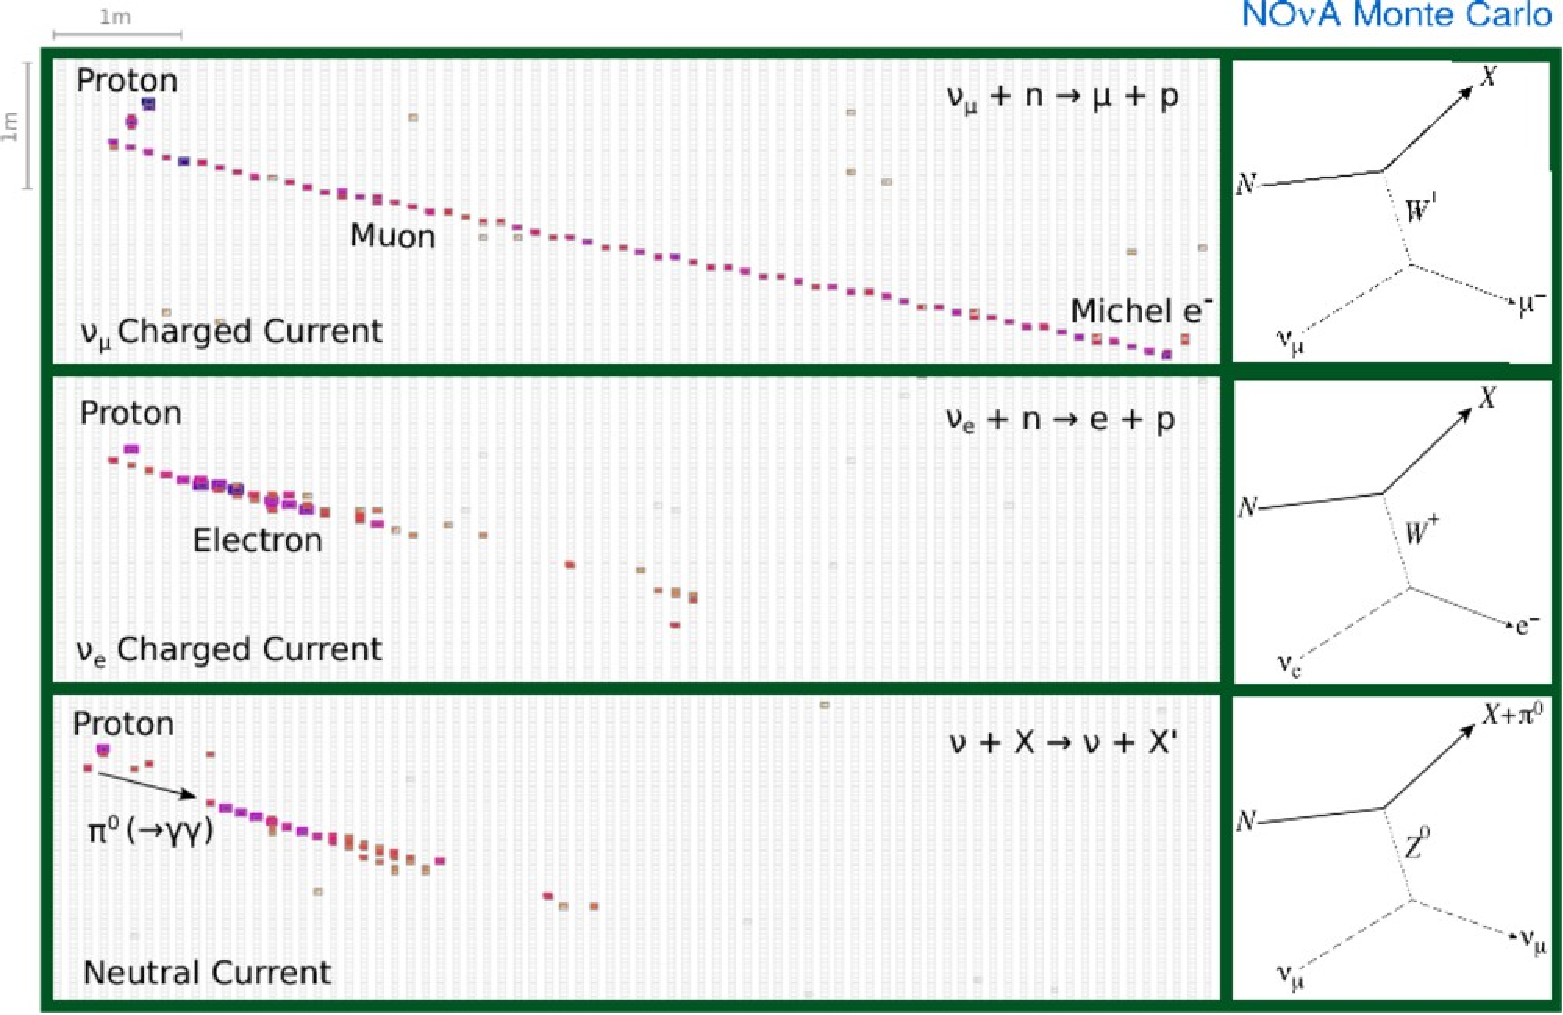
\includegraphics[width=1.0\textwidth]{figures/Det_topologies.pdf}\\%
\caption{Neutrino interactions in NOvA detectors.}
{Three types of neutrino interactions are shown. The top part shows $\nu_\mu$ CC interaction with some
proton activity and long muon track left by high energy muon. The middle part shows $\nu_e$ CC interaction,
electron develops a long electromagnetic shower with radiation length being much bigger than Moliere radius.
The bottom part shows neutrino NC interaction with $\pi^0$ among the resulting particles which later produces
an electromagnetic shower by decaying into two photons. NC type events form a primarily background in $\nu_e$
disapperance analysis.} \label{Topologies}
\end{figure}
The majority of neutrinos at the NOvA detectors are in the few GeV energy region and all the charged 
products of neutrino interaction with a nucleus are clearly visible and as long as their momenta are 
sufficiently separated in an angular space. As can been seen in \p{Topologies} muons, electrons, and charged 
hadrons leave a distinct traces in NOvA. Particles primary lose their energy through an ionization 
process by disrupting electrons of atoms which happen to be close to particles trajectories. Being 
much havier than an electron and immune to a strong interaction muon can travel a long distance inside 
the detectors which make it a relatively easy task to determine a high energy muon. Light electron interacts
with detector material via pair production and forms electromagnetic shower, where energy is depossed in 
a rather conical shaped region as opposed to a long muon track. Hadrons such as protons and pions in 
addition to ionization also lose energy by interacting strongly with nuclei along their trajectory. 

Despite these differences it is a complicated problem to distinguish a charged current (CC) interaction with 
muon or electron been produced from a neutral current (NC) one where no visible lepton is produced.
NC processes can output charged or neutral pions together with other hadrons. Charged pions
leave tracks which could be confused with low energy muons, although occasional hard scatters of the 
nuclei help with identification. Neutral pions leave electromagnetic showers after they decay into two
photons and these showers might be confused with showers created by electrons in CC neutrino interaction.
Thus, sophisticated algorithms need to be developed to measure parameters of neutrino mixing matrix where 
determination of exact neutrino flavor is a crucial task.

In addition, since NOvA Fad Detector sits on the ground it constantly being bombarded by muons and other
particles created by interactions of cosmic rays - high energy protons - with air molecules in upper atmosphere. 
These muons contribute to a background for the main analysis but they could be relatively easy to get rid off
because of their activity at the top and/or at the sides of the detector. However, they are much harder to deal
with since cosmic muons a primarily background in a uncontained sample which this thesis are partially about.

\subsection{NOvA Event Display}
\begin{figure}
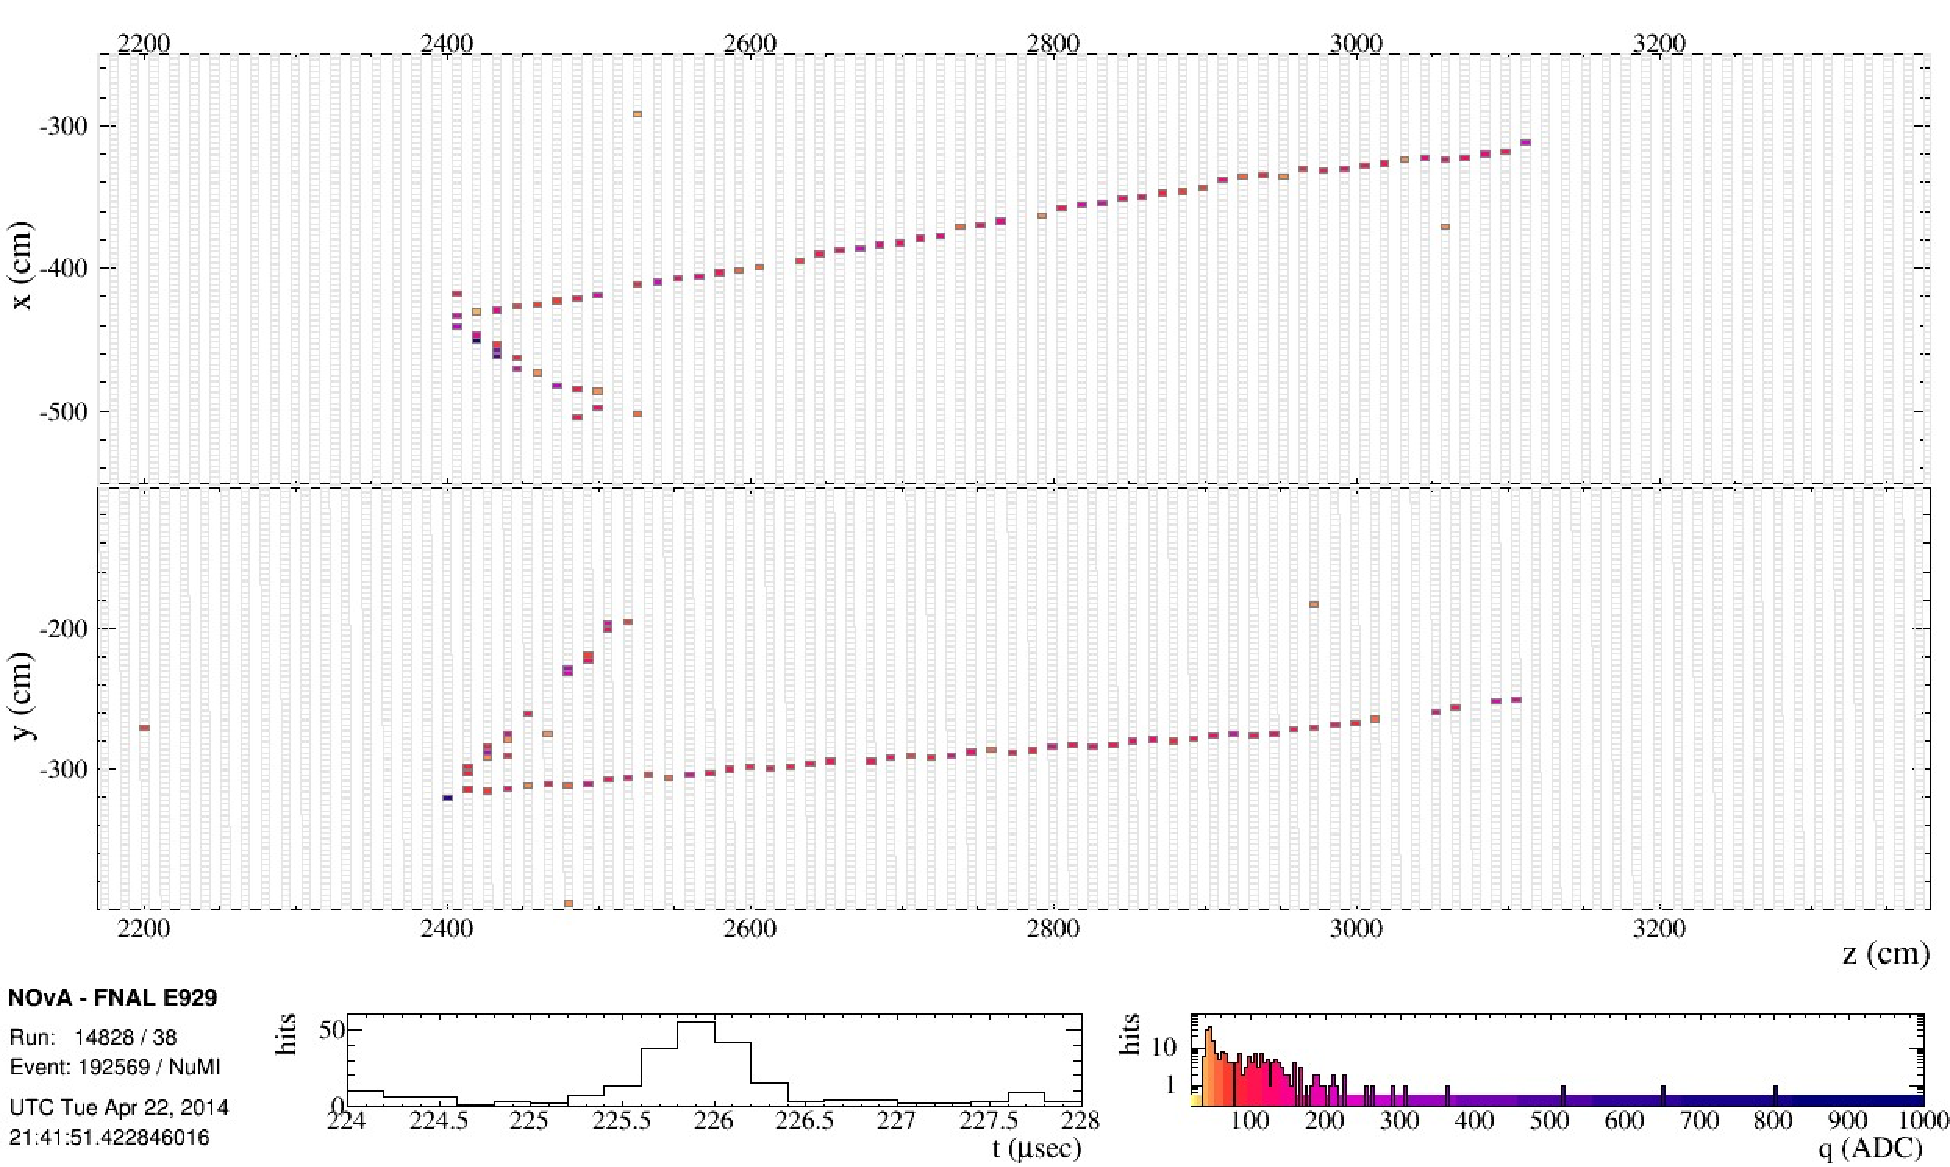
\includegraphics[width=1.0\textwidth]{figures/EventDisp.pdf}\\%
\caption{NOvA Event Display.}
{The candidate $\nu_\mu$ CC event at the Far Detector zoomed in space and time. Top and bottom windows show
X-Z and Y-Z projections.} \label{EVD}
\end{figure}
The NOvA event display helps to visualize a real data gathered by the detectors or a simulated one. The result
of $\nu_\mu$ CC interaction measured on April 22, 2014 is shown in \p{EVD}. As NOvA detectors consist of 
alternating horizontal and vertical planes, event display shows hits from two types of planes in a separate 
windows. The top window displays X-Z hits position (detector activity as seen from the top), while the lower 
one displays Y-Z hits position (detector activity as seen from the side). The software allows to change a spatial zoom as well as a time zoom to see closely activity he/she might be interested in. Hits time distribution and 
deposited photoelectron charge distribution in ADC units together with event time stamp and trigger information 
are shown below the main windows. Hits also could be colored by their time, to see if they are close to readout 
window or not, or by their deposited charge, to see where the most of the energy was deposed. In the shown 
example, hits are colored by their charge.
